% !TeX root = ../thesis.tex

\chapter{随机传值进程模型的应用}

Random VPC可以用于对云计算协议的形式刻画。
在此我们对一种云计算协议:Gossip-Style Membership Protocol进行建模和模拟实现。

\section{Gossip Style Membership协议}
\subsection{Gossip协议}
Gossip协议分为push gossip和pull gossip两种。
\begin{itemize}
   \item {
      \textbf{Push Gossip:} 
      
      消息的发送者周期性的随机选择$k$个目标节点发送Gossip Message。
      接收到Gossip Message的节点可以根据本地时间,周期性的选择$b$个目标节点发送Gossip Message。
      在发送过程中,已经拥有Gossip Message的节点仍然可以被选为目标节点。
   }
   \item {
      \textbf{Pull Gossip:}

      每个节点周期性的向$k$个目标节点发送Gossip Query,
      收到Gossip Query的节点若拥有Gossip Message的节点会向发送Query的节点返回Gossip Message的拷贝。
   }
\end{itemize}

在超过$\frac{n}{2}$的节点拥有Gossip Message时,可以证明此时选择Pull Gossip会比Push Gossip传播的更快[此处应有引用]。
因此在使用Gossip协议时,常使用Push Gossip与Pull Gossip的混合:
在消息传播$\frac{n}{2}$节点之前使用Push Gossip,在消息传播$\frac{n}{2}$之后使用Pull Gossip。

\subsection{Membership协议}

在数据中心中会频繁的出现节点的失效,
我们会为每一个节点维护一个Membership List来记录数据中心中其他节点的运行情况。
Membership Protocol是一个通过网络检测节点失效和传播失效信息的机制,
常用的Membership Protocol有Heartbeating Protocol, Gossip-Style Membership Protocol, SWIM Failure Detector Protocol等。

\section{Gossip Style Membership的实现}
\subsection{Push Gossip协议的实现}
由于Push Gossip实现难度较小,并且单一的Push Gossip协议仍然可以达到$O(\log N)$时间复杂度的消息传播,
我们以Push Gossip协议的实现作为Random VPC的demo。
其中Gossip单节点的通道示意图如图
\ref{fig1}。
以Gossip协议作为通信协议的四节点的Peer-to-Peer Sysyem的示意图如图
\ref{fig2}。

\begin{figure}[!htbp]
	\small
	\centering
	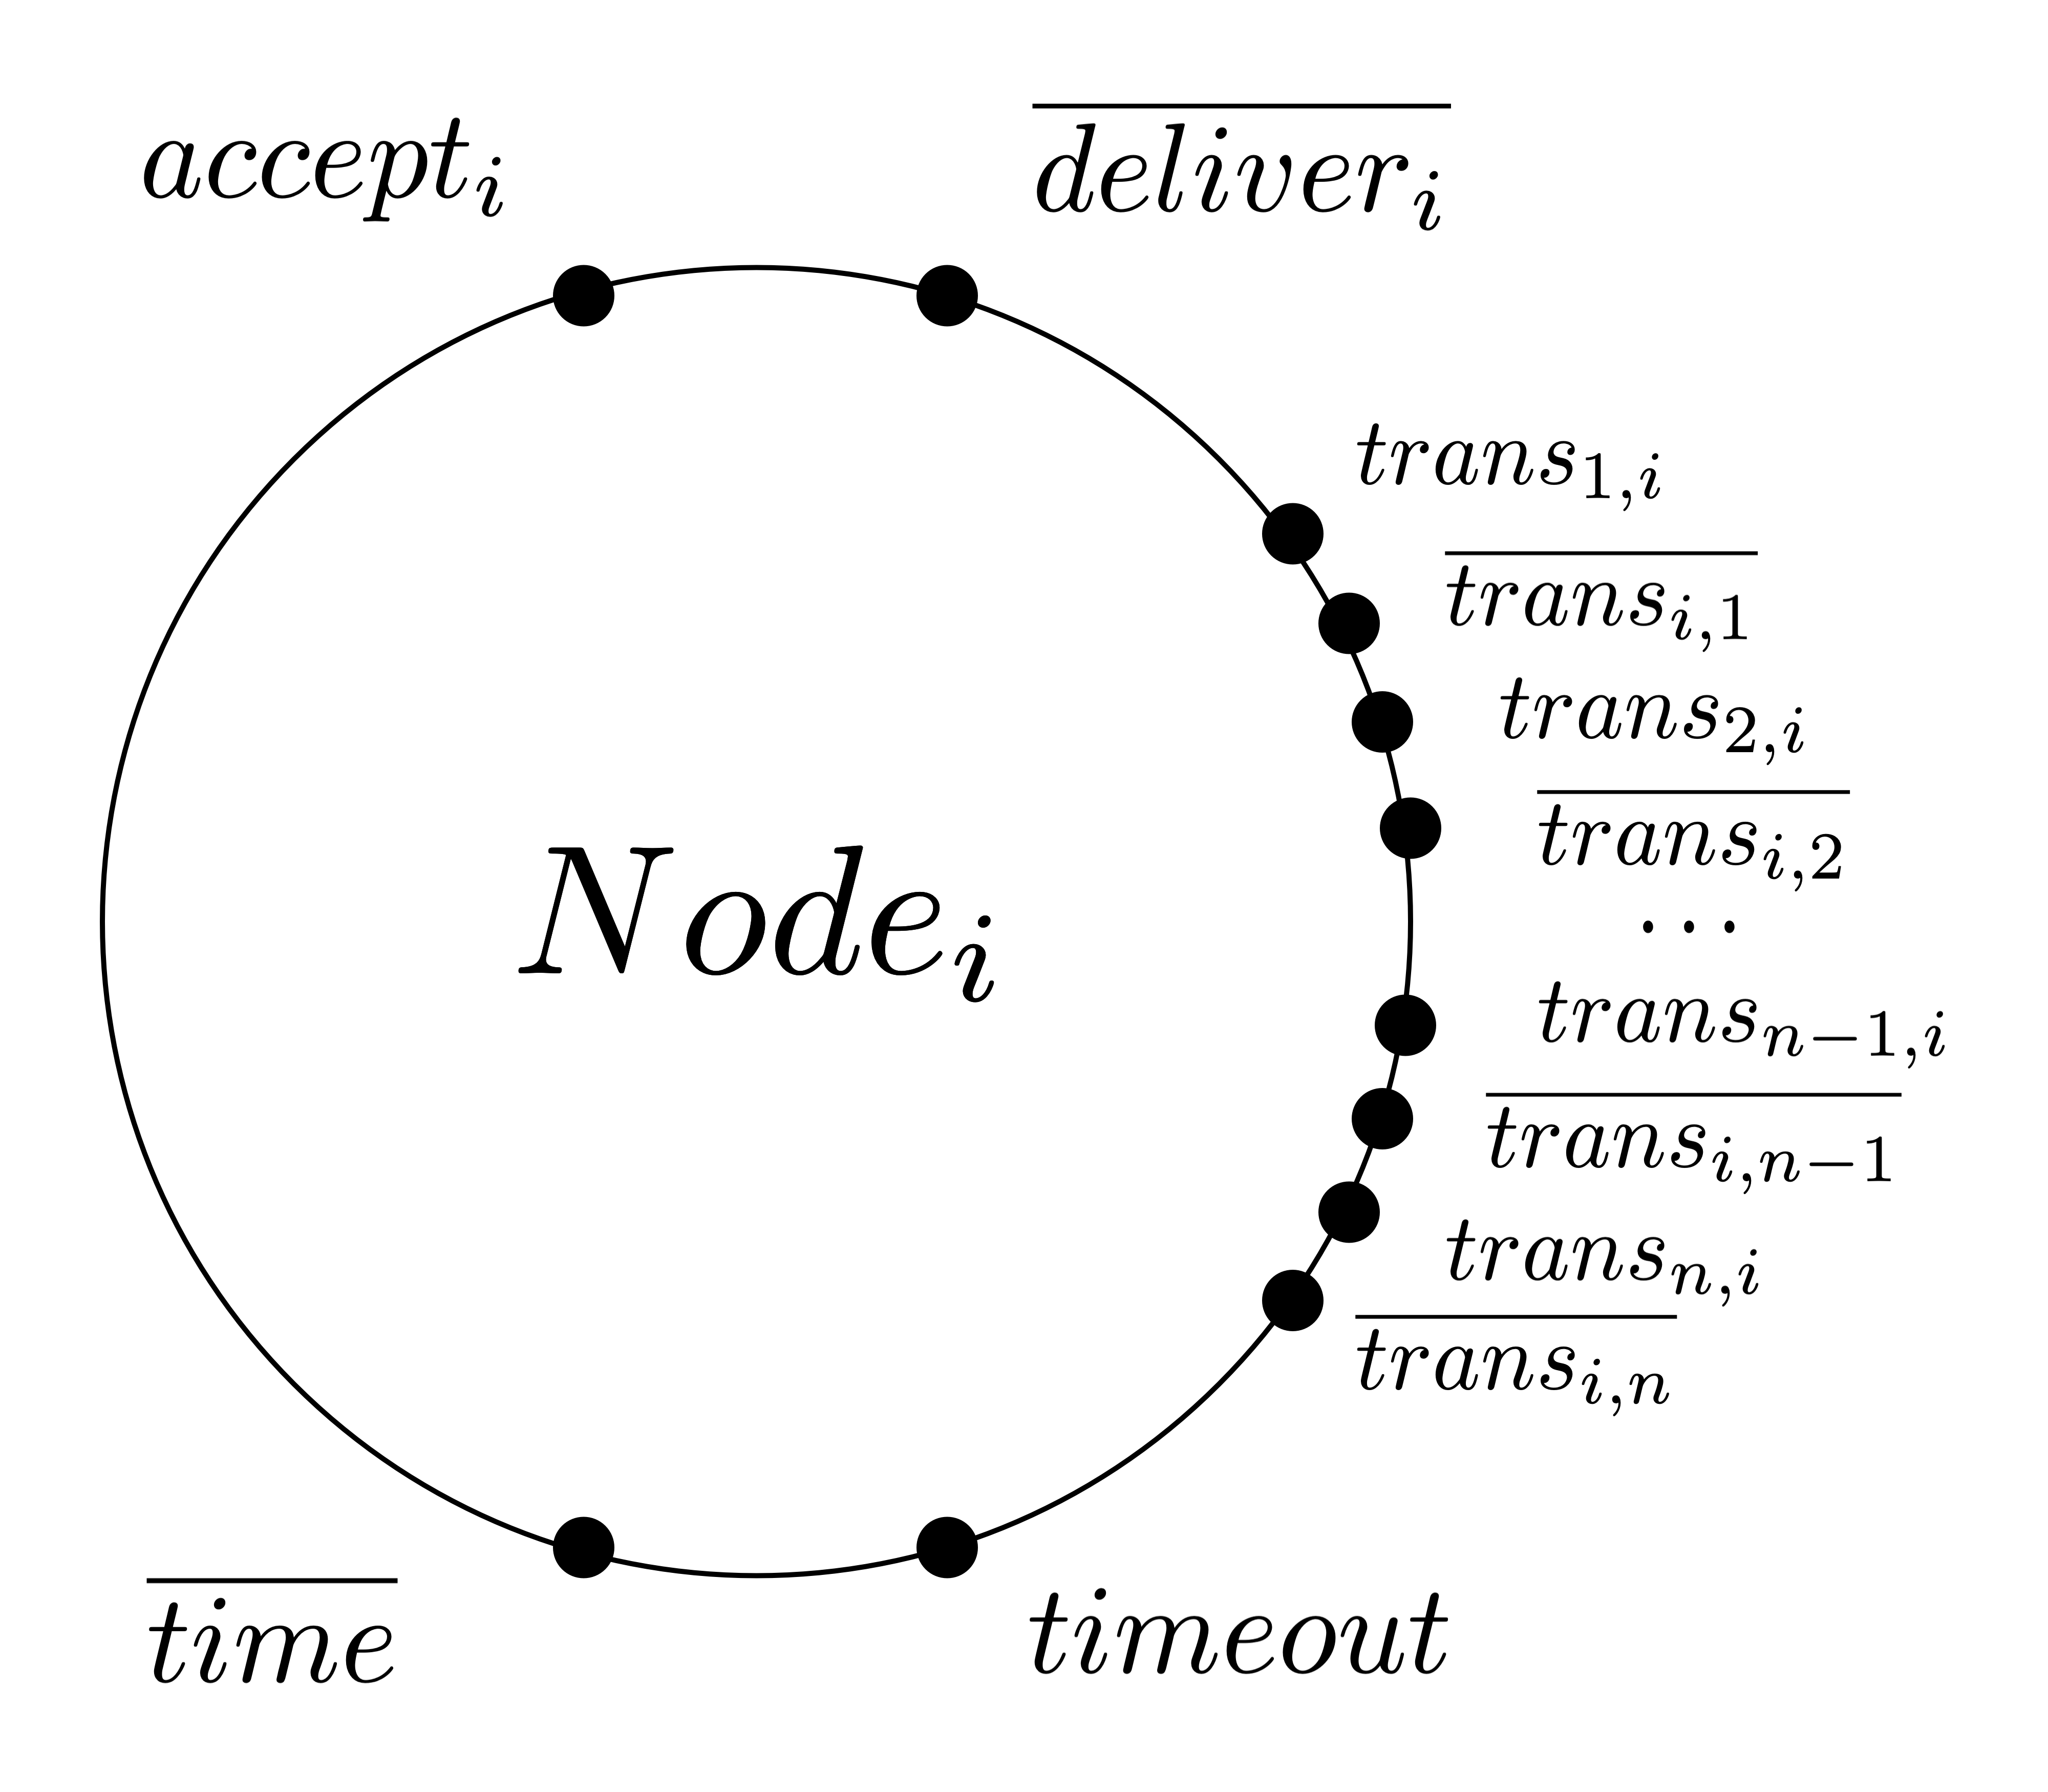
\includegraphics[width=5cm]{../figure/Node_gossip.png}
    \caption{\textbf{Gossip 节点示意图}}
    \label{fig1}
\end{figure}

\begin{figure}[!htbp]
	\small
	\centering
	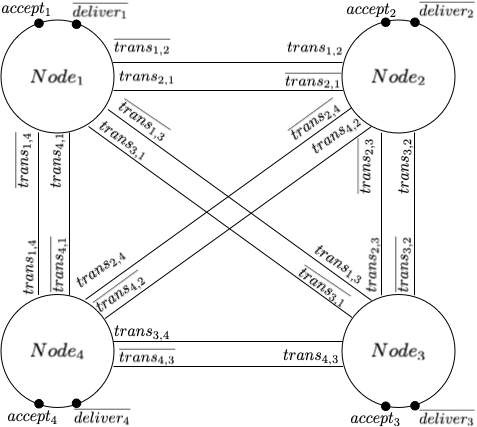
\includegraphics[width=8cm]{../figure/GossipSystem_4.png}
    \caption{\textbf{以Gossip协议作为通信协议的四节点的Peer-to-Peer Sysyem示意图(省略Timer)}}
    \label{fig2}
\end{figure}

Gossip节点Node的状态有以下几种,分别对应Gossip协议中节点的状态:
\begin{table}[!hpt]
    \caption[节点状态对应]{节点状态对应\footnotemark}
    \label{tab:firstone}
    \centering
    \begin{tabular}{@{}llr@{}} \toprule
    %   \multicolumn{2}{c}{Item} \\ \cmidrule(r){1-2}
      节点状态 & Gossip状态 \\ \midrule
      Node&可接受系统外信息(除此状态外其余均不可接受外界信息)\\
      DeliveringNode&可向系统外传递信息\\
      UnInfectiousNode&未获取Gossip Message\\
      InfectiousNode&已获取Gossip Message\\
      GossipingNode&可向系统内部特定b个其他节点发送Gossip Message\\ \bottomrule
    \end{tabular}
  \end{table}

一个基于Gossip协议的Peer-to-Peer System的定义如下。
\begin{align*}
   Node_i& \stackrel{def}{=} accept_i(x).DeliveringNode_i(x)\\
   DeliveringNode_i(x) &\stackrel{def}{=} \overline{deliver_i}(x).InfectiousNode_i(x)\\
   InfectiousNode_i(x)&\stackrel{def}{=}timeout.(\bigoplus_{perm\in \mathsf{PERM}_i} p_{perm}\tau.GossipingNode_{i,perm}(x))\\
%    &+\sum_{j\in \mathsf{N}/\{i\}}trans_{j,i}(x).DeliveringNode_i(x)\\
   GossipingNode_{i,perm}(x)&\stackrel{def}{=}\overline{trans_{i,perm_{1}}}(x).\dots \overline{trans_{i,perm_{b}}}(x).\overline{time}.InfectiousNode_i(x)\\
   UnInfectiousNode_i &\stackrel{def}{=} \sum_{j\in \mathsf{N}/\{i\}}trans_{j,i}(x).DeliveringNode_i(x)\\
   GossipSystem_\mathsf{N}&\stackrel{def}{=}(Node_1\mid UnInfectiousNode_2\mid \dots \mid UnInfectiousNode_n)\\
   &\backslash \{trans_{i,j}\mid i\in \mathsf{N} \wedge j\in \mathsf{N} \wedge i\neq j\}\cup \{time, timeout\}
\end{align*}
在这个p2p-system中共有$n$个节点,标号为$\mathsf{N}$,每一个拥有gossip message的节点周期性的向$\mathsf{k}(\mathsf{k}\leq n-1)$个其他节点发送gossip message。
其中$\mathsf{PERM}_i$为$\mathsf{N}/\{i\}$中任选$\mathsf{k}$个元素的全排列。
上述定义基于一系列理想条件的假设:
\begin{itemize}
   \item [(1)] {网络传输可靠。然而现实中的网络传输存在丢包、延迟、比特反转等问题,
   我们可以通过ACK机制来解决[此处应有引用]。对不可靠网络下的Gossip协议,我们在上述理想条件下增加对网络传输的过程的建模,建模过程在Milner的CCS中有提及[此处应有引用]。}
   \item [(2)] {节点不会损坏。在现实中节点(也就是主机)在运行了一定时间后就会宕机,对于多个节点构成的p2p系统,存在节点失效的概率只会更高[此处应有引用(MTTF)],后文的Membership协议就是来解决此类问题的。}
   \item [(3)] {系统中只存在一个消息的传输。对于单个消息源的多个消息,我们仍然可以看作单个Gossip Message一起发送;对于多个消息源,我们可以为每个节点提供消息队列机制,来保存多个消息,后文对Membership的建模提供了一个多消息源的解决思路。}
\end{itemize}

为了方便建模,我们假设一个节点选择任意其他节点作为Gossip的目标节点的概率是相同的,
即$p_{perm} = \frac{1}{A_{n-1}^{\mathsf{k}}} = \frac{(n-\mathsf{k}-1)!}{(n-1)!}$为固定值,当$\mathsf{k}=2$时,$p_{perm} = \frac{1}{(n-1)(n-2)}$。

\subsection{Push Gossip协议的等价性}

Gossip协议的目的是为了在系统内对节点进行多播,我们可以定义一个多播的Specification,同样我们只关注一个消息的多播:
\begin{definition} 单消息源的多播定义如下,其中$|\mathsf{KNOWN}|$为已经得到此消息的节点编号集合,节点可以通过$deliver$通道告知通信系统外(如本地的其他进程)节点已收到信息。
\begin{align*} 
    MulticastSpec_\mathsf{N}&\stackrel{def}{=}accept_1(x).\overline{deliver_1}(x).Multicasting_{\mathsf{N},\{1\}}(x)\\
    Multicasting_{\mathsf{N},\mathsf{KNOWN}}(x)&\stackrel{def}{=}\overline{deliver_i}(x).Multicasting_{\mathsf{N},\mathsf{KNOWN}\cup\{i\}}(x), \\
    &i\in \mathsf{N}-\mathsf{KNOWN} \wedge |\mathsf{N}|\neq |\mathsf{KNOWN}|
 \end{align*}
\end{definition} 

 \begin{definition} 为了方便后续的证明,我们给出特定状态下的$GossipSystem$的记法,其中Composition算子符合交换律。
    \begin{align*}
   &GossipSystem_{\mathsf{N},(a,b,c)}(x)\\
   &= (\stackrel{a}{\overbrace{InfectiousNode(x)\mid \dots \mid InfectiousNode(x)}}\\
   &\mid \stackrel{b}{\overbrace{DeliveringNode(x)\mid \dots\mid DeliveringNode(x)}}\\
   &\mid \stackrel{c}{\overbrace{UnInfectiousNode\mid \dots \mid UnInfectiousNode}})\\
   &\backslash \{trans_{i,j}\mid i\in \mathsf{N} \wedge j\in \mathsf{N} \wedge i\neq j\}\cup \{time, timeout\}
\end{align*}
 \end{definition} 

\begin{theorem}
    $GossipSystem_{\mathsf{N}} \approxeq^s_{\mathsf{Th}} MulticastSpec_{\mathsf{N}}$,当$\top \in \mathsf{Th}$时成立。
\end{theorem}
\begin{proof}
每一个节点能且仅能执行一次deliver操作,且deliver的顺序不影响功能,
所以我们可以规定$A\stackrel{\overline{deliver_i}(t_1)}{\longrightarrow}_{\top} B$和$C\stackrel{\overline{deliver_j}(t_2)}{\longrightarrow}_{\top}B$是互模拟的当且仅当$t_1=t_2$,对下标是否一致不作要求。
因此在后文的证明中忽略了下标。

我们可以通过构建等价集,并证明等价集是一个symbolic bisimulation关系,来证明$GossipSystem_{\mathsf{N}} \approxeq^s_{\mathsf{Th}} MulticastSpec_{\mathsf{N}}$。

构造等价集
\begin{align*}
   \mathcal{S}&=\{(GossipSystem_{\mathsf{N}}, MulticastSpec_{\mathsf{N}}), \\
      &(GossipSystem_{\mathsf{N},(n,0,0)}(x), Multicasting_{\mathsf{N},\mathsf{N}}(x))\}\\
      & \cup \{(GossipSystem_{\mathsf{N},(a,b,c)}(x), Multicasting_{\mathsf{N}, \mathsf{KNOWN}}(x))\mid |\mathsf{KNOWN}| = a\neq n\}
\end{align*}

我们来依次证明$\mathcal{S}$中的每一对等价关系为symbolic bisimulation:
\begin{itemize}
    \item {
       $GossipSystem_{\mathsf{N},(n,0,0)}(x)$和$Multicasting_{\mathsf{N},\mathsf{N}}(x)$的$\top \mathcal{S}$-tree分别只有一个根节点,
       且不能转移至其他等价集,他们的互模拟性是显然的,实际上$GossipSystem_{\mathsf{N},(n,0,0)}(x)=Multicasting_{\mathsf{N},\mathsf{N}}(x)=0$。
    }
    \item {
        对于$(GossipSystem_{\mathsf{N},(a,b,c)}(x), Multicasting_{\mathsf{N}, \mathsf{KNOWN}}(x))\mid |\mathsf{KNOWN}| = a\neq n$:

        % 对应的$Multicasting_{\mathsf{N}, \mathsf{KNOWN}}(x)\rightsquigarrow_{\top\mathcal{S}}\stackrel{\overline{deliver}(x)}{\longrightarrow}_{\top\mathcal{S}} []$
        \begin{itemize}
            \item {\textbf{Case 1: $a<n-1$。}
            $GossipSystem_{\mathsf{N},(a,b,c)}(x)$的$\top \mathcal{S}$-tree $t$如图所示:
            \begin{figure}[!htbp]
            	\small
            	\centering
            	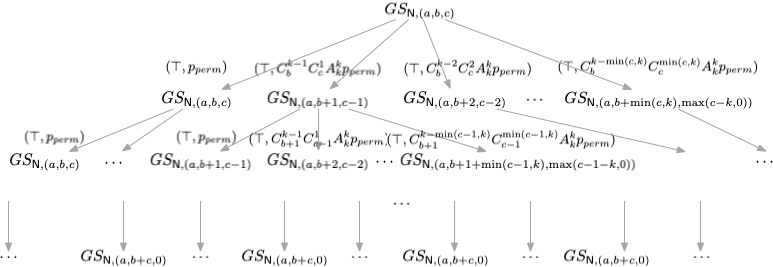
\includegraphics[width=14cm]{../figure/epsilon_tree.png}
                \caption{\textbf{$GossipSystem_{\mathsf{N},(a,b,c)}(x)$的$\top\mathcal{S}$-tree $t$}}
                \label{fig_epsilon_1}
            \end{figure}
            当$t$上的节点进入$GossipSystem_{\mathsf{N},(a,b+c,0)}(x)$状态时,
            等价的$\tau$转移就会终止,因此$GossipSystem_{\mathsf{N},(a,b+c,0)}(x)$为$t$的叶子结点。
            很显然,对$t$上的每一个非叶结点,都会经过$Node_j\stackrel{p'_j}{\rightarrow}_{\top}GossipSystem_{\mathsf{N},(a,b+c,0)}(x),p'_j=p_{j_1}p_{j_2}\dots p_{j_m}<1$。
            对$t$的叶子结点有$GossipSystem_{\mathsf{N},(a,b+c,0)}(x)\stackrel{\overline{deliver}(x)}{\longrightarrow}_{\top} GossipSystem_{\mathsf{N},(a+1,b+c-1,0)}(x)$。
            即
            $$GossipSystem_{\mathsf{N},(a,b,c)}(x)\rightsquigarrow_{\top\mathcal{S}}\stackrel{\overline{deliver}(x)}{\longrightarrow}_{\top}[GossipSystem_{\mathsf{N},(a+1,b',c')}(x)]_{\top\mathcal{S}}$$
            其中$b'+c'=b+c-1$。
            对应的我们可以用$$Multicasting_{\mathsf{N},\mathsf{KNOWN}}\rightsquigarrow_{\top\mathcal{S}}\stackrel{\overline{deliver}(x)}{\longrightarrow}_{\top} Multicasting_{\mathsf{N}, \mathsf{KNOWN}'}$$来模拟。
            对称的模拟依然成立。
            }
            \item {\textbf{Case 2: $a=n-1$。}
            \begin{itemize}
               \item {
                  {\textbf{Case 2.1:} $b=1$。}
                  $GossipSystem_{\mathsf{N},(n-1,1,0)}(x)$的$\top \mathcal{S}$-tree $t$只有一个根节点:

                  $(GossipSystem_{\mathsf{N},(n-1,1,0)}(x)\rightsquigarrow_{\top\mathcal{S}}\stackrel{\overline{deliver}(x)}{\longrightarrow}_{\top}[GossipSystem_{\mathsf{N},(n,0,0)}(x)]_{\top\mathcal{S}}$。
                  我们可以用$Multicasting_{\mathsf{N},\mathsf{KNOWN}}\rightsquigarrow_{\top\mathcal{S}}\stackrel{\overline{deliver}(x)}{\longrightarrow}_{\top} Multicasting_{\mathsf{N}, \mathsf{N}}$来模拟。
               }
               \item {
                  {\textbf{Case 2.1:} $b=0$。}
                  $GossipSystem_{\mathsf{N},(n-1,0,1)}(x)$的$\top \mathcal{S}$-tree $t$如图所示:
                  \begin{figure}[!htbp]
                     \small
                     \centering
                     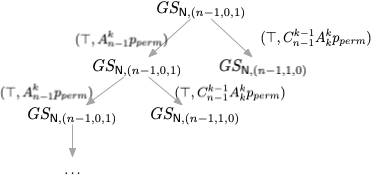
\includegraphics[width=10cm]{../figure/epsilon_tree_n-1.png}
                      \caption{\textbf{$GossipSystem_{\mathsf{N},(a,b,c)}(x)$的$\top\mathcal{S}$-tree $t$}}
                      \label{fig_epsilon_2}
                  \end{figure}
                  
                  $(GossipSystem_{\mathsf{N},(n-1,1,0)}$为$t$的叶节点。
                  因此,$(GossipSystem_{\mathsf{N},(n-1,0,1)}(x)\rightsquigarrow_{\top\mathcal{S}}\stackrel{\overline{deliver}(x)}{\longrightarrow}_{\top}[GossipSystem_{\mathsf{N},(n,0,0)}(x)]_{\top\mathcal{S}}$。
                  我们可以用$Multicasting_{\mathsf{N},\mathsf{KNOWN}}\rightsquigarrow_{\top\mathcal{S}}\stackrel{\overline{deliver}(x)}{\longrightarrow}_{\top} Multicasting_{\mathsf{N}, \mathsf{N}}$来模拟。
               }
            \end{itemize}
            }
        \end{itemize}
    }
    \item {
        对$(GossipSystem_{\mathsf{N}}, MulticastSpec_{\mathsf{N}})$,
        我们可以用$$GossipSystem_{\mathsf{N}}\stackrel{accept(x).\overline{deliver(x)}}{\longrightarrow}_{\top}GossipSystem_{\mathsf{N},(1,0,0)}(x)$$
        $$MulticastSpec_{\mathsf{N}}\stackrel{accept(x).\overline{deliver(x)}}{\longrightarrow}_{\top}Multicasting_{\mathsf{N},\{1\}}$$来相互模拟。
    }
 \end{itemize}
\end{proof}
\subsection{Gossip Style Membership的实现}

\subsubsection{Gossip Style Membership Protocol}
Gossip-Style Membership Protocol使用Gossip协议传递每个节点的Membership List。
每个节点周期性的随机选择$k$个节点发送自己的Membership List,
收到Membership List的节点根据其他节点的Membership List更新自己的Membership List。

\subsubsection{对GossipSystem的调整}
由于Gossip-Style Membership无需与外界的输入输出,并且需要提供判定和修改Membership List的函数,我们需要对之前的Gossip System进行调整。
同时,系统内的节点也会有失效的可能,我们可以用$p_{fail}$来定义一个节点失效的概率,同时经过一个内部动作$\tau$,这个节点就会被修复。
另外,由于在系统中的所有节点都是消息源,且Membership List在系统中不停的更新,因此也没有了感染者与被感染者的角色区分,
也需要对名称进行了修改。

在Gossip System节点的基础上,将原本对外暴露的$accept,deliver$通道用于连接$Membership$,作为网络中的节点获取和更新本地Membership List的通道,
修改后的节点如图
\ref{fig_membership_node}
所示。

\begin{figure}[!htbp]
	\small
	\centering
	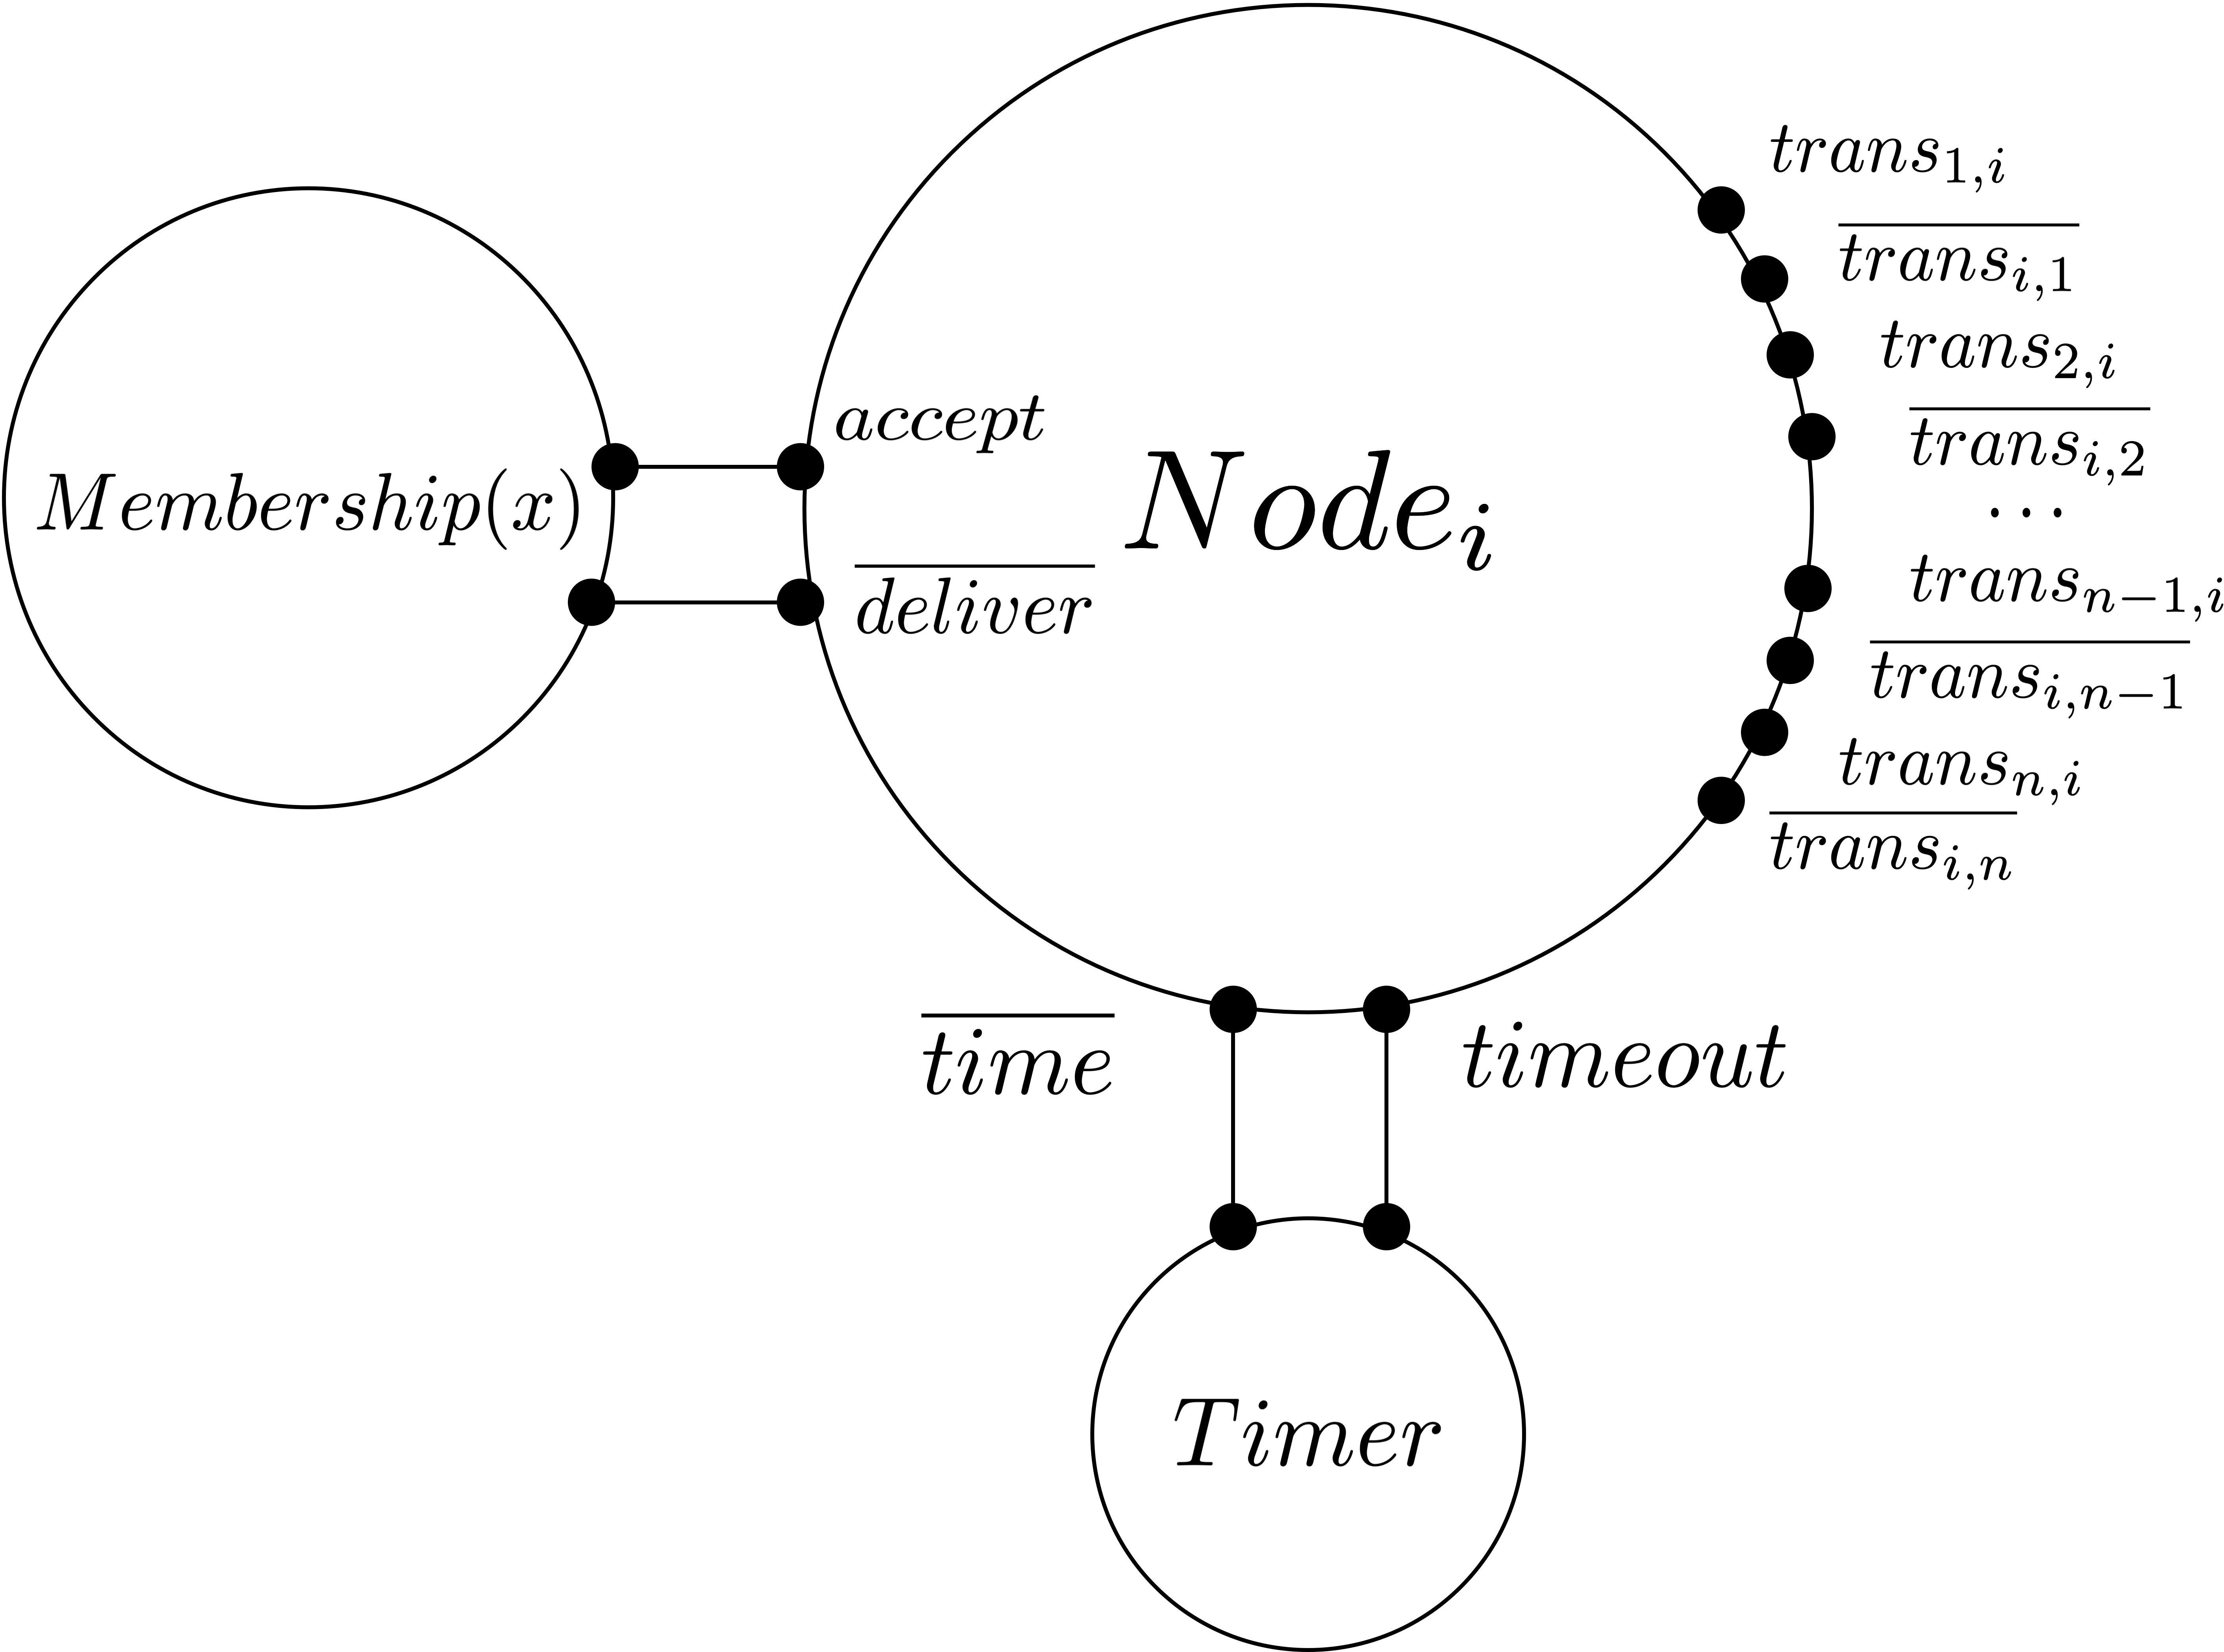
\includegraphics[width=8cm]{../figure/Node_membership.png}
    \caption{\textbf{Gossip-Style Membership Protocol 节点示意图}}
    \label{fig_membership_node}
\end{figure}
\begin{align*}
    FragileNode_i&\stackrel{def}{=}p_{fail}\tau.BadNode_i\oplus (1-p_{fail})\tau.Node_i\\
    BadNode_i&\stackrel{def}{=}\tau.FragileNode_i\\
    Node_i&\stackrel{def}{=}timeout.accept(x).(\bigoplus_{perm\in \mathsf{PERM}_i} p_{perm}\tau.GossipingNode_{i,perm}(x))\\
     &+\sum_{j\in \mathsf{N}/\{i\}}trans_{j,i}(x).\overline{deliver}(x).Node_i\\
    GossipingNode_{i,perm}(x)&\stackrel{def}{=}\overline{trans_{i,perm_{1}}}(x).\dots \overline{trans_{i,perm_{b}}}(x).\overline{time}.Node_i\\
    GossipSystem_\mathsf{N}&\stackrel{def}{=}(Node_1\mid Node_2\mid \dots \mid Node_n)\\
    &\backslash \{trans_{i,j}\mid i\in \mathsf{N} \wedge j\in \mathsf{N} \wedge i\neq j\}\cup \{time, timeout, accept, deliver\}
 \end{align*}
 其中我们需要定义Membership,来处理Membership List的获取和更新。

Membership List的内容一般为:
\begin{table}[!hpt]
    \caption[Membership List]{Membership List\footnotemark}
    \label{tab:secondone}
    \centering
    \begin{tabular}{@{}ccc@{}} \toprule
    %   \multicolumn{2}{c}{Item} \\ \cmidrule(r){1-2}
      Address & HeartBeat & Time(local) \\ \midrule
      1 & 10120 & 66\\
      2 & 10103 & 62\\
      3 & 10098 & 63\\ \bottomrule
    \end{tabular}
  \end{table}
因此Membership系统需要有一个本地计时器Timer、一个心跳计数器Counter,一个本地$MembershipList(X)$,
$X$应为一个$(Address, HeartBeat)$的二元组的数组,一个记录本地地址的$AddrInfo(address)$(地址应在加入网络时由DNS分配,此处不考虑它的分配过程)。
定义$x_i[Address]$为取Address的值的操作子,$x_i[HeartBeat]$同理。
其中$n$为MembershipList的最大容量。

Membership系统的实现如图所示:
\begin{figure}[!htbp]
	\small
	\centering
	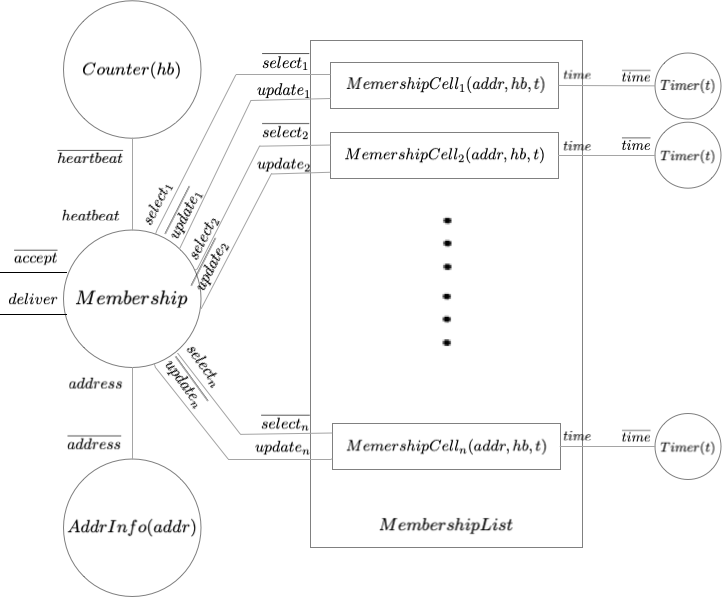
\includegraphics[width=11cm]{../figure/membership.png}
    \caption{\textbf{Membership示意图}}
    \label{fig_membership}
\end{figure}

\begin{align*}
    &Membership\stackrel{def}{=}address(addr).heartbeat(hb).select_1(x_1)\dots select_n(x_n).\\
    &\quad\overline{accept}(\{Address:addr,HeartBeat:hb\},x_1,\dots,x_n).Membership\\
    &\quad+deliver(x_1,x_2,\dots,x_n).Hashing(x_1,x_2,\dots,x_n)\\
    &Hashing(x_1,x_2,\dots,x_n)\stackrel{def}{=}(Check(x_1)\mid  \dots \mid Check(x_n) \mid Membership)\\
    &Check(x)\stackrel{def}{=}address(addr).((addr=x[Address])0|\urcorner(addr=x[Address])Find_1(x))\\
    &FindAndUpdate_i(x)\stackrel{def}{=}select_i(x_i).(\\
    &\quad(x_i = \epsilon) (\overline{update_i}(x).0)\\
    &\quad| \urcorner(x_i = \epsilon)(\\
    &\quad(x_i[Address]=x[Address])(\\
    &\quad(x_i[HeartBeat]<x[HeartBeat])(\overline{update_i}(x).0)\\
    &\quad\mid \urcorner (x_i[HeartBeat]<x[HeartBeat])0)\\
    &\quad\mid \urcorner (x_i[Address]=x[Address])FindAndUpdate_{i+1}(x))),i\leq n\\
    &FindAndUpdate_i(x)\stackrel{def}{=}0,i>n
   \end{align*}
   \begin{align*}
    &MembershipCell_i(addr,hb,t)\stackrel{def}{=}\\
    &\quad\overline{select_i}(\{Address:addr,HeartBeat:hb\}).MembershipCell_i(addr,hb,t)\\
    &\quad+update_i(\{Address:addr',HeartBeat:hb'\}).time(t').MembershipCell_i(addr',hb',t')\\
    &MembershipList\stackrel{def}{=}(MembershipCell_1(\epsilon)\mid \dots MembershipCell_n(\epsilon))\\
    &AddrInfo(addr)\stackrel{def}{=}\overline{address}(addr)\\
    &Counter(hb)\stackrel{def}{=}\overline{heartbeat}(\mathsf{s}(hb)).Counter(\mathsf{s}(hb))
\end{align*}
其中$\mathsf{s}(x)$表示$\mathsf{s}(x)=x+1$[此处应有引用]。
\section{Gossip-Style Membership的仿真模拟}
在本章节我们会根据本章的模型来实现一个Gossip-Style Membership Protocol,
由于资源限制,不能实际部署在多个主机构成的集群,我们将使用多进程来模拟多个主机。

\subsection{Go语言与CSP}
我们将使用Go语言实现Gossip-Style Membership Protocol,
Go语言实现了两种并发模型,一种是C++,Java使用的多线程,一种是CSP并发模型。

CSP与CCS存在相似和差异[引用],本实现主要利用了Go语言的通道特性,
通道的概念是CSP的组成部分,在CCS中对应port的概念,其本质是相似的。
使用Go语言的通道可以更加直观的展示出对上述模型的代码实现。

\subsection{说明与实现效果}
本节仿真实现的Gossip-Style Membership Protocol参数如下:
\begin{table}[!hpt]
   \caption[Gossip-Style Membership Protocol仿真参数]{Gossip-Style Membership Protocol仿真参数\footnotemark}
   \label{tab:thirdone}
   \centering
   \begin{tabular}{@{}ccc@{}} \toprule
   %   \multicolumn{2}{c}{Item} \\ \cmidrule(r){1-2}
     参数名称 & 参数值 & 参数含义 \\ \midrule
     $n$ & 8 & 系统节点数量\\
     $k$ & 2 & Gossip协议中每次感染的其他节点数\\
     $p_{fail}$ & 0.1 & 节点失效概率\\ \bottomrule
   \end{tabular}
 \end{table}